\chapter{Translation: Four Letters, Twenty Amino Acids}

\begin{kaichang}
Find three things in your refrigerator: tofu, an egg, and milk. One comes from soybeans, one from a hen, one from a cow, with vastly different colors, smells, and textures. But send each to a laboratory for ``complete hydrolysis,'' breaking all its proteins apart, and you obtain almost identical inventories: the same roughly twenty amino acids, no more and no fewer.

The reverse works too. Eat tofu for lunch, and soybean proteins break into amino acids in your gut. Hours later, muscle cells may have reassembled those amino acids into human muscle protein. Soy protein becomes your protein: shared raw materials, separate blueprints.

Now guess. Messenger RNA writes protein blueprints with only four ``letters,'' but must specify twenty amino acids. Is one letter per amino acid enough? Two? How many letters did life settle on per group? Are extra combinations waste or useful? We will return to the tofu with answers at the end.
\end{kaichang}

\section{Phenomena: Twenty Bricks, Countless Buildings}

First, describe measurable facts without rushing to explain.

Fact one: protein variety is enormous, ingredient variety tiny. Hair keratin, egg-white ovalbumin, digestive enzymes, and antiviral antibodies (Chapter 61) differ completely in properties, yet full hydrolysis yields the same list of twenty amino acids (Chapter 48). This list crosses species: E. coli, elephants, mushrooms, and you use the same bricks. What differs is their \textbf{sequence}.

Fact two: protein production is astonishingly fast. In good conditions, E. coli divides every twenty minutes, requiring a fresh copy of its millions of protein molecules within that time. Your body is no slouch: hundreds of grams of old protein are broken down and replaced daily. Muscle, plasma proteins, and enzymes continually renew.

Fact three is surprising: the machinery can be removed for study. Gently disrupt cells and centrifuge them, and the resulting ``cell-free extract'' still synthesizes proteins in a tube when supplied with amino acids and energy. Protein synthesis is not mysterious whole-organism magic but machinery whose parts can be separated and examined. This test-tube phenomenon opens our evidence story later.

Fact four lies on your plate. Your body cannot make eight or nine of the twenty amino acids and must obtain them ready-made from food: ``essential amino acids.'' This is the entire meaning of nutritional ``protein quality.'' Tofu's strength is not its flavor but its amino-acid list matching your needs. Long-term extreme dietary restriction often leaves particular bricks missing, not merely insufficient total ``protein.'' The production line has blueprints and machines, but lacks materials.

Fact five: tiny sequence differences can greatly change properties. Pig and human insulin differ by just one amino acid, allowing early pig-pancreas insulin to treat people. Some genetic diseases, such as sickle-cell anemia, involve a single amino-acid substitution in a protein that changes the chain's folding and properties. Protein information lies in sequence, not its ingredient list. That is the weight behind ``translation'': order must be transmitted faithfully, letter by letter.

\section{Particles: Messenger, Carriers, Assembly Bench}

Zoom to molecules. Chapter 68 described RNA polymerase copying DNA into portable messenger RNA (mRNA), bearing four nucleotide letters, A, U, G, and C. But amino acids do not recognize bases. Mix mRNA and amino acids and nothing happens: one speaks ``nucleotide,'' the other lacks even that alphabet. A translator must connect the languages.

Life employs two roles:

\begin{itemize}[itemsep=2pt]
\item \textbf{tRNA: a carrier that reads at one end and carries cargo at the other}. A short RNA folds into a specific shape. One end exposes three nucleotides, the \textbf{anticodon}, recognizing three mRNA letters by complementary pairing (Chapter 66's A with U, G with C). The other end holds a specific amino acid. It is a living dictionary between languages.
\item \textbf{Aminoacyl-tRNA synthetase: the loading supervisor}. Amino acids do not climb onto the right tRNA themselves. Each amino acid has a dedicated enzyme that loads it onto matching tRNA using ATP. This is translation's first accuracy checkpoint: load the wrong cargo, and perfect reading afterward is useless.
\end{itemize}

Finally comes the assembly bench, the \textbf{ribosome}. Ribosomal RNA (rRNA) and dozens of proteins form large and small subunits, like two mold halves holding mRNA between them. The ribosome performs translation's central task: matching amino-acid-bearing tRNAs to positions and catalyzing peptide bonds. Crucially, its catalytic core is mainly RNA, not protein: essentially an RNA enzyme. This is a major clue in Chapter 56's origin-of-life discussion: working RNA may be older than proteins.

\begin{center}
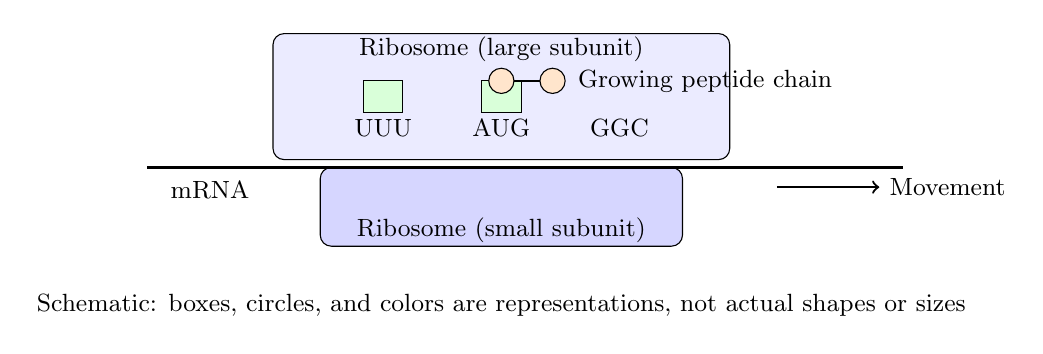
\begin{tikzpicture}[scale=1]
\draw[rounded corners, fill=blue!8] (1.6,0.55) rectangle (7.4,2.15);
\node at (4.5,1.95) {\small Ribosome (large subunit)};
\draw[rounded corners, fill=blue!16] (2.2,-0.55) rectangle (6.8,0.45);
\node at (4.5,-0.35) {\small Ribosome (small subunit)};
\draw[thick] (0,0.45) -- (9.6,0.45);
\node[below] at (0.8,0.4) {\small mRNA};
\node at (3.0,0.95) {\small UUU};
\node at (4.5,0.95) {\small AUG};
\node at (6.0,0.95) {\small GGC};
\draw[->, thick] (8.0,0.2) -- (9.3,0.2) node[right] {\small Movement};
\draw[fill=green!15] (2.75,1.15) rectangle (3.25,1.55);
\draw[fill=green!15] (4.25,1.15) rectangle (4.75,1.55);
\draw[fill=orange!20] (4.5,1.55) circle (0.16);
\draw[fill=orange!20] (5.15,1.55) circle (0.16);
\draw[thick] (4.66,1.55) -- (4.99,1.55);
\node[right] at (5.35,1.55) {\small Growing peptide chain};
\node[align=center] at (4.5,-1.3) {\small Schematic: boxes, circles, and colors are representations, not actual shapes or sizes};
\end{tikzpicture}
\end{center}

Translation is therefore \textbf{information recoding}: four-letter mRNA sequences become twenty-brick amino-acid sequences through tRNA adapters on ribosome assembly benches. What are the recoding rules? How many letters specify an amino acid?

\section{Rules: Three Letters Make a Word}

This is the chapter's most beautiful step, requiring only multiplication.

One letter per amino acid permits four possibilities, short of twenty. Two-letter groups give $4\times 4=16$, still insufficient. Three give $4\times 4\times 4=64$, exceeding twenty for the first time. Thus \textbf{triplets are the shortest scheme able to encode twenty amino acids}. Nature's answer is indeed three: three consecutive mRNA nucleotides form a \textbf{codon}, specifying an amino acid.

Reading has three further experimentally established rules: start at a fixed point; read consecutive, \textbf{nonoverlapping} triplets; and use no commas or spaces. Misplace the start and everything afterward fails. Shift the reading frame by one letter and it is like shifting the three-character groups in the Chinese saying ``Three monks have no water to drink'' by one character: the resulting broken word groups turn the whole message into gibberish. This is a \textbf{frameshift}, far more damaging than one misspelled letter. Chapter 72 revisits its cost.

\begin{qiaoliang}
There are 64 boxes for twenty amino acids and three ``stop signals.'' Are the extra 41 wasted? Quite the opposite: they cushion errors. Several codons often specify the same amino acid: glycine has four ``synonyms,'' serine six. This is code \textbf{degeneracy}. Synonyms usually differ at the third letter while their first two remain fixed. That has practical consequences: replication or transcription errors (inevitable, as Chapter 67 explained) in the third position often leave the amino acid unchanged. The code ``absorbs'' the error. Life did not pursue costly zero-error performance; it made coding insensitive to mistakes. Engineering repeatedly uses the same exchange of redundancy for robustness.
\end{qiaoliang}

Codons also have special jobs. The \textbf{start codon}, AUG, both fires the starting gun, setting the frame, and codes for methionine. Nearly every new polypeptide therefore begins with methionine, which may later be removed. Three \textbf{stop codons}, UAA, UAG, and UGA, specify no amino acid; they are full stops.

\section{Symbols: The Code Table}

Now introduce the symbols. The complete genetic code has 64 boxes, available in any biochemistry textbook. Here are representative entries; notice patterns rather than memorizing boxes.

\begin{table}[htbp]
\centering
\begin{tabular}{lll}
\toprule
Codons & Meaning & Comment \\
\midrule
AUG & Methionine & \shortstack[l]{Also starts translation\\and sets the frame} \\
UUU, UUC & Phenylalanine & \shortstack[l]{Differ only at\\the third position} \\
UAU, UAC & Tyrosine & \shortstack[l]{Differ only at\\the third position} \\
GGU, GGC, GGA, GGG & Glycine & \shortstack[l]{Any third\\letter works} \\
\shortstack[l]{UCU, UCC, UCA,\\UCG, AGU, AGC} & Serine & \shortstack[l]{Up to six\\synonyms} \\
UAA, UAG, UGA & Stop & \shortstack[l]{Specify no\\amino acid} \\
\bottomrule
\end{tabular}
\end{table}

Here is pairing in symbols. mRNA codons are read $5'$ to $3'$; tRNA anticodons run oppositely and complement them:

\[ \text{mRNA codon}\ 5'\text{-AUG-}3' \quad \longleftrightarrow \quad \text{tRNA anticodon}\ 3'\text{-UAC-}5' \]

Amino acids join through Chapter 48's peptide bond, a \chem{-CO-NH-} linkage formed by removing water between one amino acid's amino group and the preceding amino acid's carboxyl group. Inside ribosomes, the essential step transfers the old peptide chain from its tRNA onto the amino acid carried by the incoming tRNA. Successive peptide bonds lengthen the chain. We are discussing information, but information never comes free: every step carries Chapter 50's energy bill, which we will calculate shortly.

Here is how to read a full code table without fear: rows and columns organize a codon's first, second, and third bases. Look up coordinates on a map: locate the first base, then the second, then the third within the box to find the amino acid. Try GGU: first G and second G locate glycine; any third letter stays in that box. The table layout makes degeneracy visible.

\section{The Line: Start, Extend, Finish}

With components and rules, the line runs like this:

\textbf{Initiation}. The small ribosomal subunit binds mRNA and slides to the first AUG. Initiator tRNA carrying methionine matches its anticodon; the large subunit closes over it, completing the bench. The reading frame is now locked.

\textbf{Elongation}. A three-step cycle adds one amino acid per turn: (1) Entry: loaded tRNA tries its seat and is rejected if the anticodon mismatches, the second proofreading checkpoint. (2) Bond formation: the ribosome transfers the whole existing chain to the new amino acid by forming a peptide bond. (3) Translocation: the ribosome moves three letters along mRNA, clearing cargo space for the next seat.

\textbf{Termination}. A stop codon enters the seat, but no tRNA claims it: the cell provided no carriers for these three codons. Instead, a protein \textbf{release factor} arrives, detaches the polypeptide, and allows the subunits to separate. Parts are recycled for the next mRNA.

How accurate is the line? Very, but never perfect. Loading enzymes can select the wrong amino acid; anticodons can misread. After layered checks, total translation errors are about one per ten thousand incorporated amino acids. Compare Chapter 67's DNA replication at roughly one per billion. Why the difference? Think of cost. A faulty polypeptide wastes one chain, which can be replaced; a faulty DNA copy alters the master blueprint inherited by all that cell's descendants. Proofreading costs energy and time, and precision investment matches error consequences. Energy and probability are governing the accounts again.

How fast? Bacterial ribosomes add around twenty amino acids per second; your cells add several per second. A 300-amino-acid chain takes one ribosome roughly fifteen seconds to a minute. Several ribosomes often work simultaneously along one mRNA, like beads threaded on wire: a polyribosome. Thousands or tens of thousands of benches working continuously sustain those hundreds of grams of daily protein renewal.

\begin{qiaoliang}
Keep an honest energy account. Adding an amino acid costs roughly four ``ATP equivalents'': loading converts ATP to AMP (two equivalents), while entry and translocation each use one GTP. Estimate adult daily protein synthesis at $300$ grams and average residue mass at $110$ daltons. That means roughly $2.7$ moles of peptide bonds daily, about $1.6\times 10^{24}$ bonds. Multiply by four and use approximately $50$ kilojoules per mole of ATP hydrolyzed: daily protein synthesis costs around $500$ kilojoules, a few percent of total energy use. Even lying still all day, your body continuously pays for ``information becoming matter.'' You may challenge every input---synthesis amount, energy price---and recalculate with figures you find yourself.
\end{qiaoliang}

\section{Evidence: Cracking the Code}

\begin{zhengju}
After the double helix appeared in 1953, the next question was obvious: how do four letters specify twenty amino acids?

One of the first to calculate seriously was physicist Gamow. He derived ``at least triplets'' and proposed an elegant hypothesis: adjacent codons overlap, sharing letters. This predicts that changing one amino acid must affect neighbors and restrict possible protein sequences. As more sequences became available, those restrictions were absent. The hypothesis was decisively rejected. Beautiful theories must yield to data.

Meanwhile, in 1955 Crick made a bolder prediction: amino acids cannot directly recognize bases, so cells must contain an ``adapter,'' recognizing code at one end and carrying amino acid at the other. Nobody had seen it. A few years later, tRNA was found, strikingly matching the predicted form and function. Like Mendeleev's empty boxes, prediction before discovery is a theory's strongest moment.

Experiments actually opened the table. In 1961, Crick and Brenner used chemicals inserting or deleting single DNA bases. Insert one letter: the gene fails. Insert two: still fails. Insert three: function largely returns! This directly supports triplets read continuously from a fixed start. That same year, Nirenberg and Matthaei added synthetic all-U RNA (poly-U) to a cell-free protein-making system. The tube produced only one ``protein,'' a pure phenylalanine chain. The first codon was deciphered: UUU = phenylalanine. The control was clear: without that RNA, nothing was synthesized. Over subsequent years, Khorana and others synthesized known repeating sequences, such as UCUCUC…, producing alternating serine and leucine chains, and filled the table box by box. By 1966, all 64 codons were established.

Notice the story's shape: mathematical reasoning, rejected hypotheses and confirmed predictions, then clever controlled experiments filling each box. No step leapt straight to the answer by ``genius intuition.''
\end{zhengju}

\section{Boundaries: Translation Is Not Completion}

The code-table-and-production-line model answers ``in what order do amino acids go?'' It cannot answer the chain's shape, job, or destination. A newly released polypeptide usually is not ready to work:

\begin{itemize}[itemsep=2pt]
\item \textbf{It must fold}. Chapter 48's rules give a specific three-dimensional form, sometimes assisted by chaperone proteins. Misfolded chains are tagged, dismantled, and recycled.
\item \textbf{It needs modifications}. Many proteins must lose a segment (insulin begins as a long chain and becomes active after an intervening segment is removed), gain sugar chains, or receive phosphates (Chapter 58's phosphorylation switches) before completion.
\item \textbf{It needs transport}. An initial ``signal peptide'' often acts as a shipping address for mitochondria, cell membrane, or secretion. Even excellent protein cannot reach its post with the wrong address.
\end{itemize}

Another boundary concerns information: the code specifies ``what,'' not ``how much.'' An mRNA may be translated once or thousands of times. Actual protein abundance depends on mRNA quantity, lifetime, and translation rate, none specified by the code table. That gap opens the next chapter.

\begin{shiyan}
\textbf{Be a Ribosome on Paper.}

Materials: paper, pen, and this chapter's partial codon table.

Steps: (1) Copy this mRNA, reading from $5'$: AUGGGUUUUCACUAA. (2) Start at the first AUG, divide into triplets, look up each, and write the amino-acid sequence. (3) Mutate the sixth letter G to A, translate again, and compare sequences. (4) Make a harsher change: insert A after the fourth letter, regroup, and translate again. Where does the disruption begin, and how far does it go?

Observations: In step (3), did changing GGU to GGA alter the amino acid? This is degeneracy's cushion. In step (4), why is one extra letter more damaging than one changed letter?

Safety: A paper-only activity; the only danger is miscounting boxes. If you miscount, start again: a ribosome would not lose count.
\end{shiyan}

\begin{wuqu}
``The genetic code is universally shared, unchanging, and exceptionless.'' The first part is almost right: bacteria and elephants share a dictionary, strong evidence of common ancestry. But ``no exceptions'' is wrong. Your mitochondria, descendants of ancient bacteria, privately changed several rules: UGA means stop in cytoplasm but tryptophan in human mitochondria. More remarkably, under specific conditions UGA can encode the twenty-first amino acid, selenocysteine, found in your antioxidant enzymes. Some ciliates reassign stop codons too. The code is an evolutionary product, not a physical law, and evolutionary products bear traces of change. This matters beyond exams: moving a gene under the ``standard code'' into a different-code expression system can produce the wrong product, a pitfall revisited in Chapter 84.
\end{wuqu}

\section{Back to the Tofu}

Now fulfill the opening promise. One letter specifies only four possibilities, two only sixteen, both short of twenty. Three give 64, enough for the first time, so life uses triplets. Extra boxes are not wasted: three serve as full stops, the others as error-cushioning synonyms.

Why do tofu, eggs, and milk differ so much? Soybeans, hens, and cows have different mRNA sequences, giving different amino-acid orders, folded shapes, textures, smells, and nutrition. Why are their ingredients interchangeable, allowing tofu to become human muscle? They share twenty amino-acid building blocks and the same dictionary. Your gut recognizes bricks, not buildings: dismantle someone else's blueprints and direct new ribosomal construction with your mRNA. Information, not matter, separates you from tofu.

\section{Beyond the Assembly Bench}

Understanding the mechanism immediately explains several important things.

First, medicine. Erythromycin ointment in your medicine cabinet and prescribed tetracycline target ribosomes. These antibiotics jam particular bacterial ribosome sites, stopping translation. Your ribosomes differ enough that the same dose leaves them largely unaffected: the molecular basis of ``killing bacteria without harming the body.'' Dose and individual variation still matter, of course, and antibiotics cannot distinguish harmful bacteria from Chapter 62's friendly gut tenants. Misuse also selects resistant bacteria, natural selection's bill (Chapter 76).

\textbf{Translator safety note:} Selective targeting does not mean antibiotics are harmless: side effects can be serious, and medicines are not interchangeable. Use antibiotics only as directed, take them exactly as prescribed, and ask a clinician or pharmacist about adverse effects; see \href{https://www.cdc.gov/antibiotic-use/about/}{CDC antibiotic guidance}.

Conversely, the ribosome is a vulnerable point. Diphtheria bacteria can be deadly because their toxin ``locks'' your ribosomes, shutting down translation. One indispensable line for every protein provides both efficiency and vulnerability.

Next, evolution. Mitochondria have their own ribosomes, resembling bacterial rather than cytoplasmic ribosomes in both size and antibiotic sensitivity. Evidence of their ancient bacterial ancestry is engraved on their assembly benches (Chapter 56's endosymbiosis story).

Then engineering. With a nearly universal code, transfer a human insulin gene into bacteria and they faithfully translate human insulin. Most insulin used by people with diabetes today is made this way; Chapter 83 explains how the route became workable.

Leave a larger question pending: a cell has tens of thousands of genes, so should every available line translate at full speed? Nerve and muscle cells carry the same DNA, yet make completely different protein lineups. Who chooses which mRNAs are made, how many, and how long they last? The bench executes orders; command lies elsewhere. Chapter 70 examines genes being switched on, turned down, and switched off. Codon synonyms leave another account open too: changing a DNA letter sometimes leaves protein untouched. Is this ``silent change'' an error, material, or innovation? Chapter 72 will tell.

\begin{tiaozhan}
How many errors can degeneracy absorb? Calculate it yourself. Every codon has nine single-letter changes: three positions, each with three replacements. For GGU (glycine), changing the third base (GGU$\rightarrow$GGC, GGA, GGG) never changes meaning; changing the first or second almost certainly gives another amino acid. Check all $64\times 9=576$ single-letter changes, and about a quarter leave amino acids unchanged, even before counting gentler substitutions with chemically similar amino acids. The code places shock absorbers at position three. Why there? Think about which codon--anticodon pairing position has the loosest requirements, called ``wobble.'' You may skip this section without losing the thread.
\end{tiaozhan}

\section*{Try It Yourself}

\begin{sikaoti}
\item Draw the flow of information from DNA to a finished protein. Include mRNA, tRNA, aminoacyl-tRNA synthetase, and ribosome. At each arrow, identify the language, the recoding agent, and where energy is spent.
\item Translate AUGUAUGGCUAA from $5'$ using this chapter's table. Then shift the reading frame one position, regroup, and describe what happens.
\item A bacterial ribosome adds about twenty amino acids per second. How long does a 500-amino-acid chain take? At four ATP equivalents per addition, approximately how many ATP equivalents does it cost?
\item Could alien life encode twenty amino acids with five nucleotide letters in two-letter groups? Compare advantages and costs with our four-letter, three-per-group system. (Hint: consider combinations, codon totals, and degeneracy's buffering.)
\item Why does erythromycin block bacterial ribosomes without directly shutting down your cells? Why, nevertheless, can prolonged broad-spectrum antibiotic use cause gastrointestinal discomfort? Use Chapter 62's ecosystem view.
\item Design an experiment to test ``AAA encodes lysine.'' What artificial mRNA and reaction system would you use, which product would you observe, and what controls would you set?
\end{sikaoti}
